
\chapter{Implementación}
\label{chap:implementación}

La idea no es implementar un sistema production ready, pero si verificar que as comunicaciones funcionan correctamente. En este capitulo describiremos la implementación de las capas de conocimiento y nivel del bucle. Dejaremos para más adelante, el capitulo \ref{chap:caso_estudio} la descripción de la implementación del nivel de solución y sistema manejado. En este capitulo ofrecemos una vista más concreta de la implementación, y las tecnologías empleadas. EN el otro describiremos cómo encaja todo a nivel general y veremos cómo opera.

Una vez descrito el diseño del sistema, llegamos a la etapa de implementación. Aunque no era uno de los objetivos del trabajo, optamos por implementar un sistema básico que siga el diseño. De esta forma pudimos verificar la distribución de los componentes, verificar la viabilidad de los conectores y refinar los protocolos de comunicación. La implementación fue incremental, y el diseño fue evolucionando según detectábamos nuevas necesidades o problemas que no resolvía nuestra arquitectura. Así pudimos validar qué funcionaba y que no.

La implementación se llevo a cabo en 4 hitos distintos, cada uno correspondiente a una etapa distinta del bucle:
\begin{itemize}
  \item \textbf{Hito 1 - Servicio de monitorización y conocimiento}
  \item \textbf{Hito 2 - Servicio de análisis y reglas}
  \item \textbf{Hito 3 - Planificador}
  \item \textbf{Hito 4 - Ejecutor y efectores}
\end{itemize}

\section{Servicio de monitorización y conocimiento}

En esta primera etapa acordamos implementar el proceso de registro de las medidas de una sonda, hasta que se graba en el conocimiento. Esto implicó implementar las sondas y monitores del caso de estudio (capitulo \ref{chap:caso_estudio}), el componente de monitorización del bucle MAPE-K y la base de conocimiento. Se comenzó también con el prototipado de los que se convertirían en los conectores para comunicaciones descendentes: los conectores de APIs REST.

El objetivo era implementar desde que la sonda reporta una medida hasta que se almacena esta nueva medida en el conocimiento. Para ello tuvimos que implementar la comunicación entre la sonda y el monitor de la solución. Después del monitor de la solución al componente de monitorización del bucle. Y de este último al conocimiento. La implementación de todos ellos fue muy parecida.

Respecto a los servicios, se optó por implementar el sistema con servicios en ASP.NET\footnote{Página oficial: \url{https://docs.microsoft.com/en-us/aspnet/core/introduction-to-aspnet-core}}. Se trata de un \emph{framework} para implementar servidores web de la plataforma .NET de Microsoft. Como comentamos en la sección \ref{chap:OpenAPI}, estos servicios expondrán \foreign{english}{endpoints} HTTP. En el listing \ref{ls:csharp-get} ya mostramos un ejemplo de la implementación de estos \foreign{english}{endpoints}.

A partir de estos endpoints, gracias al uso de la librería \emph{Swashbuckle.AspNetCore}\footnote{Página oficial: \url{https://github.com/domaindrivendev/Swashbuckle.AspNetCore}}, pudimos generar la especificación de nuestros servicios en el estándar OpenAPI. Esto nos aporta dos cosas: una interfaz de usuario para interactuar con la API y la posibilidad de generar el API client.

Hablemos primero sobre la interfaz de usuario. La librería añade a nuestro servicio el \emph{endpoint} \texttt{/swagger}. Accediendo a esta ruta, el servicio nos presentará una interfaz con un listado de todas las operaciones que ofrece la API Rest. De cada petición nos muestra su documentación (la que añadimos en el código), sus parámetros y nos permite incluso ejecutarla allí mismo. De esta forma, nuestros usuarios pueden hacer pruebas de las peticiones antes de implementar su propio cliente. O para situaciones de emergencia cuando necesitemos ejecutar una petición por algún motivo (depuración?)

\begin{figure}[htb]
  \centering
  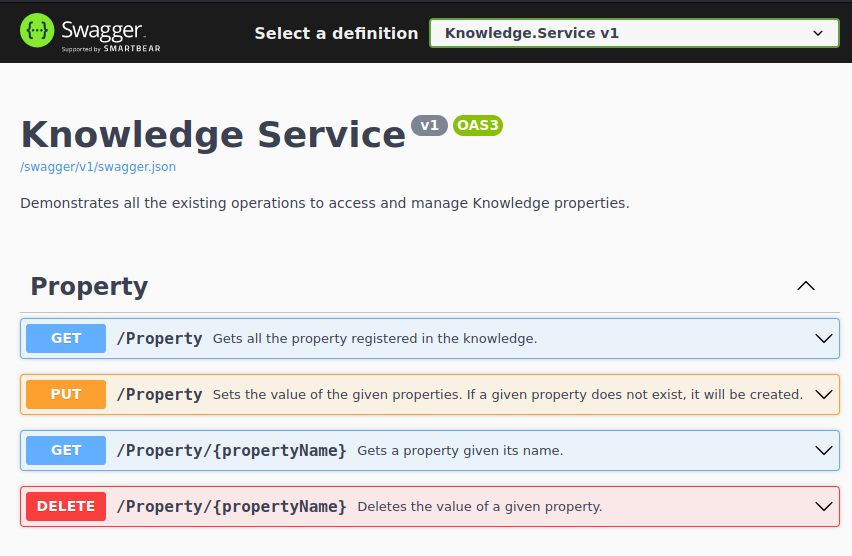
\includegraphics[scale=1.5]{cap_implementacion/images/swagger-knowledge-ui}
  \caption{Interfaz de usuario ofrecida por Swagger para el servicio de conocimiento. Se genera a partir de las especificación OpenAPI.}
  \label{fig:swagger-knowledge-ui}
\end{figure}

Por otro lado, también nos permite generar el API Client. Como comentamos en la sección de OpenAPI, tenemos gran variedad de generadores de código a nuestra disposición. Nosotros optamos por los ofrecidos por la librería \texttt{OpenApi.Generators}\footnote{Página del proyecto: \url{https://github.com/OpenAPITools/openapi-generator}}. En concreto, el generador de código de \verb|C#|. Usándolo, pudimos generar una librería que permite contactar con nuestro servicio, sin necesidad de implementar mucho código. Por ejemplo, el componente de monitorización del bucle contacta a través del bucle MAPE-K a través del API Client generado.

El módulo del conocimiento es un servicio muy sencillo. Para esta implementación de referencia optamos por implementarlo con un diccionario en memoria, que asigna los pares clave-valor. Esto nos permite direccionarlas y acceder desde fuera a estos recursos. Ofrece operaciones de lectura y escritura sobre estas propiedades y configuraciones de servicio.

Por encima de este, tenemos el módulo de monitorización. Actúa como intermediario entre los monitores de la solución y el conocimiento. También cuenta con una implementación muy sencilla. Ofrece operaciones de lectura de propiedades del conocimiento y para los monitores de la solución reporten medidas. De esta forma, los monitores de solución podrán obtener los valores de otras propiedades y valor si deben permitir o no la escritura de esa medida.

\textcolor{red}{¿Añadir ejemplo? ¿Desribir los componentes implementados? ¿Debería describirse el caso de uso con la implementación del bucle MAPE-K?}

\section{Servicio de análisis y reglas}
\label{sec:implementacion-modulo-reglas}

En el segundo hito, acordamos implementar la evaluación de reglas de adaptación. Esto requería de implementar el módulo de análisis del bucle MAPE-K y los módulos de reglas de la solución. En este hito empezamos a plantearnos el diseño de las comunicaciones ascendentes: las notificaciones. Con ellas, evitaríamos que se los componentes se acoplaran a la capa superior.

Primero describiremos las notificaciones. Optamos por implementar estas operaciones con \texttt{RabbitMQ}\footnote{Página oficial: \url{https://www.rabbitmq.com/}}. Se trata de un \foreign{english}{broker} de mensajería ''sencillo'' ampliamente utilizado. \cite{newmanBuildingMicroservicesDesigning2021} Nos permitió implementar los dos patrones de comunicación que necesitamos: las notificaciones y las peticiones asíncronas.

Para implementar nuestro conector, utilizamos una librería llamada \texttt{Rebus}\footnote{Página oficial: \url{https://github.com/rebus-org/Rebus}}. Esta nos permite interactuar con un bus, abstrayéndonos de la tecnología concreta utilizada para la comunicación. Así, podríamos cambiar de tecnología de transporte en cualquier momento por otra que se ajuste más a nuestros requisitos.

Finalmente, para desacoplar la funcionalidad de los servicios de la publicación y consumición de mensajes del bus, empleamos \texttt{MediatR}\footnote{Página oficial: \url{https://github.com/jbogard/MediatR}}. Esta librería ofrece un mediador que nos permite propagar eventos dentro de un servicio. El emisor no necesita tener referencias a los receptores. Es similar a un \foreign{english}{broker} de mensajería, pero interproceso.

Comentado esto, describiremos la implementación de la comunicación entre el módulo de conocimiento y el servicio de análisis. Una vez se confirma la escritura de una propiedad o configuración en el conocimiento, este propaga internamente un \textbf{evento de integración} (línea 11 del fragmento \ref{ls:knowledge-set-property}) a través del mediador.


\begin{lstlisting}[language={[Sharp]C},caption={Implementación del método que asigna valor a una propiedad. Muestra un ejemplo de propagación interna de eventos de integración.},captionpos=b, label=ls:knowledge-set-property]
private async Task SetProperty(SetPropertyDTO propertyDto)
{
    var newValue = new()
    {
        Value = propertyDto.Value,
        LastModification = DateTime.UtcNow,
    };

    properties.AddOrUpdate(propertyDto.Name, newValue, (_, _) => newValue);

    await _mediator.Send(
      new PropertyChangedIntegrationEvent(propertyDto.Name));
}

\end{lstlisting}

El mediador le pasará el evento a nuestro publicador. Este publicará en el exchange el evento  (línea 15 del fragmento \ref{ls:knowledge-property-changed-publisher}). Lo recibirán todos los suscriptores ubicados en la capa superior.

\begin{lstlisting}[language={[Sharp]C},caption={El publicador de eventos captura el evento de integración que se propaga internamente, y lo publica en el bus.},captionpos=b, label=ls:knowledge-property-changed-publisher]
public class PropertyChangedIntegrationEventPublisher
  : IIntegrationEventPublisher<PropertyChangedIntegrationEvent>
{
  private readonly IBus _bus;

  public PropertyChangedIntegrationEventPublisher(IBus bus)
  {
      _bus = bus;
  }

  public async Task<Unit> Handle(
      PropertyChangedIntegrationEvent notification,
      CancellationToken cancellationToken)
  {
      await _bus.Publish(notification);

      return Unit.Value;
  }
}
\end{lstlisting}

Finalmente, en el servicio de análisis, tenemos el consumidor (fragmento \ref{ls:analysis-property-changed-consumer}). Este recibirá el evento del bus y lo propagará internamente en el servicio. De esta forma, todos los manejadores (\foreign{english}{handlers}) del evento lo recibirán y podrán tratarlo.

\begin{lstlisting}[language={[Sharp]C},caption={El consumidor recibe el evento de integración del bus y lo propaga internamente. Todos los manejadores de este evento lo recibirán.},captionpos=b, label=ls:analysis-property-changed-consumer]
public class PropertyChangedIntegrationEventConsumer
  : IIntegrationEventConsumer<PropertyChangedIntegrationEvent>
{
  private readonly AnalysisServiceDiagnostics _diagnostics;

  private readonly IMediator _mediator;

  public PropertyChangedIntegrationEventConsumer(
      AnalysisServiceDiagnostics diagnostics,
      IMediator mediator)
  {
      _diagnostics = diagnostics;
      _mediator = mediator;
  }

  public async Task Handle(PropertyChangedIntegrationEvent message)
  {
      using var activity = _diagnostics.PropertyChangeEventReceived(message);

      await _mediator.Publish(message);
  }
}
\end{lstlisting}

En cuanto a la implementación del módulo de análisis, este realmente no tiene mucha lógica. Participa como intermediario entre el conocimiento y los módulos de reglas. Recibe los eventos de cambios en las propiedades y los propaga a la capa superior, usando el tópico correspondiente. Esto nos permitió abstraer a las reglas del acceso al conocimiento, y limitar su acceso solo a lecturas de propiedades y configuración.

En trabajos posteriores, este servicio podría ampliarse añadiendo autenticación y autorización. Así, se podría evitar que servicios no autorizados accedan al conocimiento o soliciten adaptaciones maliciosas.

Respecto a la implementación de los módulos de reglas, ofrecemos una implementación de referencia. Como estos se encuentran a nivel de la solución, el desarrollador es libre de elegir la que considere más conveniente.

En el fragmento \ref{ls:adaption-rule-base} mostramos la clase base para implementar reglas de adaptación. Vemos que esta clase está suscrita a los eventos de integración de cambio de propiedad de adaptación y cambio en la configuración del sistema (lineas 2-3). Cuando el consumidor capture uno de estos eventos, lo propagará internamente y todas las reglas afectadas lo capturarán.

Esta clase base se desarrolló siguiendo el patrón plantilla (o \foreign{english}{template})\footnote{\url{https://refactoring.guru/design-patterns/template-method}}. Ofrece un método que evalúa la condición de la regla (\texttt{EvaluateCondition}) y, si esta se cumple, la ejecuta (\texttt{Execute}). Las reglas que hereden de esta deberán implementar ambos métodos.

\begin{lstlisting}[language={[Sharp]C},caption={Clase base para implementar reglas de adaptación. Se evalúa la condición, y si esta se cumple, se ejecuta.},captionpos=b, label=ls:adaption-rule-base]
public abstract class RuleBase
    : IIntegrationEventHandler<PropertyChangedIntegrationEvent>,
      IIntegrationEventHandler<ConfigurationChangedIntegrationEvent>
{
    // ..

    private async Task Handle()
    {
        try
        {
            if (await EvaluateCondition())
            {
                await Execute();
            }
        }
        catch (Exception e)
        {
            _diagnostics.RuleEvaluationError(_ruleName, e);

            throw;
        }
    }

    protected abstract Task<bool> EvaluateCondition();

    protected abstract Task Execute();

    // ..
}
\end{lstlisting}

Respecto a las suscripciones, las herederas deberán indicar de qué propiedades o claves de configuración dependen. En base a ellas, deberemos suscribirnos a las notificaciones que emite el módulo de análisis. Para ello, hemos implementado una serie de atributos que permiten declarar estas dependencias.

En el fragmento \ref{ls:adaption-rule-dependencies} mostramos un ejemplo. En la línea 1 tenemos el atributo que describe las dependencias con la propiedad de adaptación \texttt{Temperature}. Por otro lado, en las líneas 2-5 tenemos la declaración de dependencias con dos claves de configuración del servicio \texttt{Climatisation.AirConditioner}: \texttt{TargetTemperature} y \texttt{Mode}.

\begin{lstlisting}[language={[Sharp]C},caption={Las reglas declaran sus dependencias sobre propiedades de adaptación usando atributos. Estos se utilizarán para las suscripciones a los temas de los eventos.},captionpos=b, label=ls:adaption-rule-dependencies]
[RuleKnowledgePropertyDependency(ClimatisationConstants.Property.Temperature)]
[RuleServiceConfigurationDependency(
    ClimatisationAirConditionerConstants.AppName,
    ClimatisationAirConditionerConstants.Configuration.TargetTemperature,
    ClimatisationAirConditionerConstants.Configuration.Mode)]
public class DisableAirConditionerWhenCoolingAndTargetTemperatureAchievedAdaptionRule
  : AdaptionRuleBase
{
    // ...
}
\end{lstlisting}

Para suscribirnos a las notificaciones de cambio de las dependencias de las reglas utilizaremos la \textbf{reflexión}: analizaremos el ensamblado del servicio buscando todas las reglas y obtendremos los valores de sus atributos. En base a ellos, nos suscribiremos a los \foreign{english}{topics} en el \foreign{english}{broker} de mensajería.

\begin{lstlisting}[language={[Sharp]C},caption={Para suscribirnos a los \foreign{english}{topics} de las notificaciones obtenemos las dependencias de las reglas mediante reflexión},captionpos=b, label=ls:rules-registration]
public static IServiceCollection AddAdaptionLoopAnalysisServices(
  this IServiceCollection services,
  IConfiguration configuration,
  Assembly rulesAssembly)
{
    // ...

    services.AddBus(
        configuration,
        rulesAssembly,
        registerSubscriptions: async bus =>
        {
            var subscriptions = GetRulesBusTopicNames(rulesAssembly);

            foreach (var subscription in subscriptions)
            {
                await bus.Advanced.Topics.Subscribe(subscription);
            }
        });

    return services;
}
\end{lstlisting}

\section{Planificador}

En el tercer hito implementamos las peticiones de cambio de las reglas y el servicio de planificación. Aquí surge también la necesidad de un tercer patrón de comunicación: las peticiones asíncronas.

Continuando por donde nos quedamos, una vez se evalúa la condición de la regla y esta estima que debe ejecutarse, necesitamos un mecanismo para solicitar cambios en la configuración del sistema. En el cuerpo de la regla se solicitarán cambios a la configuración actual del sistema en base a los síntomas que haya detectado la regla. En el fragmento \ref{ls:change-request-builder} mostramos un ejemplo de esta solicitud de cambio. Para un síntoma determinado, \texttt{TemperatureGreaterThanHotThreshold} (línea 6), requerimos que el servicio \texttt{Climatisation.AirConditionerService} esté presente (lineas 7-10) con la configuración \texttt{Mode} con el valor \texttt{Cooling} (lineas 11-13).

\begin{lstlisting}[language={[Sharp]C},caption={Implementación de la misma petición siguiendo el patrón \emph{builder}.},captionpos=b, label=ls:change-request-builder]
protected override async Task Execute()
{
  await _systemService.RequestConfigurationChange(changeRequest =>
  {
    changeRequest
      .ForSymptom(TemperatureGreaterThanHotThreshold)
      .WithService(ClimatisationAirConditionerConstants.AppName, service =>
      {
        service
          .MustBePresent()
          .WithParameter(
            ClimatisationAirConditionerConstants.Configuration.Mode,
            AirConditioningMode.Cooling.ToString());
      });
  });
}
\end{lstlisting}

Las reglas comunicarán esta solicitud de cambio al módulo de análisis. Esta solicitud de cambio deberá comunicársela al módulo de análisis, que la redirigirá al planificador. Este deberá generar un \textbf{plan de cambio} a partir de las solicitudes.

Para redirigir esta petición de cambio, usaremos las peticiones asíncronas. Su implementación es muy similar a la de las notificaciones, explicada en detalle en el apartado anterior. La única diferencia radica en la cardinalidad de la comunicación: el módulo de análisis publicará el mensaje directamente en la cola de trabajo, en lugar de publicarlo en un exchange para que lo reciba cualquier subscriptor. Entonces, sólo cambia la implementación del publicador. En la línea 14 del fragmento \ref{ls:request-publisher} vemos que el mensaje se enruta directamente a la cola \texttt{PlanningServiceQueue}.

\begin{lstlisting}[language={[Sharp]C},caption={Para suscribirnos a los \foreign{english}{topics} de las notificaciones obtenemos las dependencias de las reglas mediante reflexión},captionpos=b, label=ls:request-publisher]
public class SystemConfigurationChangeRequestPublisher
  : IRequestPublisher<SystemConfigurationChangeRequest>
  where TRequest : Request
{
  public SystemConfigurationChangeRequestPublisher(IBus bus)
  {
      _bus = bus;
  }

  public async Task<Unit> Handle(
      SystemConfigurationChangeRequest request,
      CancellationToken cancellationToken)
  {
      await _bus.Advanced.Routing.Send(
          AdaptionLoopPlanningConstants.Queues.PlanningServiceQueue,
          request);

      return Unit.Value;
  }
}
  \end{lstlisting}

El resto de la implementación será muy similar. Solo cambiará las interfaces que debamos implementar para cada tipo de componente (\texttt{IRequestConsumer} en lugar de \texttt{IIntegrationEventConsumer}, etc.).

El planificador recibirá esta petición de cambio y deberá elaborar un plan de adaptación. Para ello, verificará que el plan de cambio es viable. En nuestro prototipo, para reducir el ámbito del proyecto, nos limitamos a comprobar que la configuración sea distinta a la configuración actual. Si el sistema ya se encuentra en el estado solicitado, el plan de cambio se queda vacío y no se propaga.

Para ello, el servicio de planificación compara la configuración actual con la solicitada, y añade al plan de adaptación las \textbf{acciones de adaptación} requeridas para alcanzar el estado deseado. Ya comentamos que los operadores arquitectónicos con los que operaremos serán del ámbito de los microservicios: activar servicio, eliminar servicio, vincular servicios, desvincularlos y cambiar su configuración.

Por ejemplo, un plan de adaptación para la regla evaluada anteriormente sería:

\begin{lstlisting}[language=python,caption={Plan de adaptación generado. Solo contiene una acción de adaptación: cambiar la configuración \texttt{Mode} del servicio \texttt{AirConditioner}.},captionpos=b, label=ls:adaption-change-plan]
{
  "ChangePlan": {
    "Timestamp": "2022-07-09T09:53:01.1868834Z",
    "Actions":
    [
      {
        "Type": 3, // Set Parameter
        "ServiceName": "Climatisation.AirConditioner.Service",
        "PropertyName": "Mode",
        "PropertyValue": "Cooling"
      }
    ]
  },
  "Symptoms":
  [
    {
      "Name": "temperature-lesser-than-cold-threshold",
      "Value": "true"
    }
  ]
}
\end{lstlisting}

\section{Ejecutor y efectores}

En el hito final implementamos el módulo ejecutor y los efectores. Este módulo recibirá el plan de adaptación del planificador. A partir de este, deberá distribuir las acciones de adaptación que contiene entre sus servicios de efectores.

Para transmitirle el plan de adaptación del planificador al ejecutor, volvemos a recurrir a las peticiones asíncronas. De forma similar al servicio de análisis y el planificador, estos se encuentran en la misma capa. El plan de adaptación que se le pasa como evento de integración es el que ya mostramos en el fragmento \ref{ls:adaption-change-plan}.

Una vez captura la petición, el ejecutor deberá determinar qué servicios debe cambiar, y manipular sus efectores. Para nuestra implementación, simplemente agrupamos las acciones por el nombre del servicio afectado. Las publicaremos como notificaciones usando el nombre del servicio como tema.

Estas notificaciones las capturan los servicios de efectores.
La comunicación entre el módulo de planificación  y el ejecutor. El efector actúa como un traductor del modelo de alto nivel al nivel del sistema: \textcolor{red}{citar paper de garlan} para cada acción de adaptación, deberá determinar cómo ejecutarla en el sistema manejado. Estos servicios son los que manipularán el estado del sistema. Actúan como envoltorios del mismo. La comunicación entre este servicio y el sistema es un tanto especial: dependerá del sistema manejado; de si tenemos control sobre su implementación. Si no es así, tendremos que adaptarnos a la implementación que ofrezca este (HTTP, mensajería...).

Dependiendo de la acción, el efector hará una acción u otra: deplegar un servicio, o eliminarlo, cambiar la configuración, etc.

Continuando con nuestro ejemplo del modo del aire acondicionado, el sistema modificaría la configuración del mismo. Una vez se confime el cambio, si se ha llevado a cabo, se ejecutará actualizará su valor en la base de conocimiento. Dependerá de si el sistema es capaz de hacerlo o debe recaer la responsabilidad en el efector.
